% This work is made available under the terms of the
% Creative Commons Attribution-ShareAlike 4.0 license,
% http://creativecommons.org/licenses/by-sa/4.0/.
%
% Version: $Revision$

\documentclass[a4paper]{book}

\usepackage{wrapfig}
\usepackage{graphicx}
\usepackage{hyperref}
\usepackage{multirow}
\usepackage{scalefnt}
\usepackage{tikz}
\usepackage{varwidth}

% watermark -- for draft stage
\usepackage[firstpage]{draftwatermark}
\SetWatermarkLightness{0.9}
\SetWatermarkScale{5}

% Copyright (c) 2009 by the University of Waikato, Hamilton, NZ. 
% This work is made available under the terms of the 
% Creative Commons Attribution-ShareAlike 3.0 license, 
% http://creativecommons.org/licenses/by-sa/3.0/. 
%
% Version: $Revision$

\newenvironment{tight_itemize}{
\begin{itemize}
  \setlength{\itemsep}{1pt}
  \setlength{\parskip}{0pt}
  \setlength{\parsep}{0pt}}{\end{itemize}
}

\newenvironment{tight_enumerate}{
\begin{enumerate}
  \setlength{\itemsep}{1pt}
  \setlength{\parskip}{0pt}
  \setlength{\parsep}{0pt}}{\end{enumerate}
}

% if you just need a simple heading
% Usage:
%   \heading{the text of the heading}
\newcommand{\heading}[1]{
  \vspace{0.3cm} \noindent \textbf{#1} \newline
}

\newcommand{\icon}[1]{\tikz[baseline=-3pt]\node[inner sep=0pt,outer sep=0pt]{\includegraphics[height=1.1em]{#1}};}


\title{
  \textbf{ADAMS} \\
  {\Large \textbf{A}dvanced \textbf{D}ata mining \textbf{A}nd \textbf{M}achine
  learning \textbf{S}ystem} \\
  {\Large Module: adams-net} \\
  \vspace{1cm}
  
\includegraphics[width=2cm]{images/net-module.png} \\
}
\author{
  Peter Reutemann
}

\setcounter{secnumdepth}{3}
\setcounter{tocdepth}{3}

\begin{document}

\begin{titlepage}
\maketitle

\thispagestyle{empty}
\center
\begin{table}[b]
	\begin{tabular}{c l l}
		\parbox[c][2cm]{2cm}{\copyright 2012-2016} &
		\parbox[c][2cm]{5cm}{
\includegraphics[width=5cm]{images/coat_of_arms.pdf}} \\
	\end{tabular}
	
\includegraphics[width=12cm]{images/cc.png} \\
\end{table}

\end{titlepage}

\tableofcontents
\listoffigures
%\listoftables

%%%%%%%%%
% Email %
%%%%%%%%%

\chapter{Email}
Flows are ideal for being run as background jobs (``-headless'' flag). For
example, importing or processing data in batches can be done at night time. 
Of course, you want to be notified if something went wrong or some predictions
are off. Adding the \textit{SendEmail} sink to existing flows, allows for automatic
sending of emails that were generated by the \textit{CreateEmail} transformer: 
if everything is OK then send an email to the customer,
otherwise send an email to sysadmin. The \textit{CreateEmail} actor adds all incoming
file names, e.g., the array output of a \textit{DirectoryLister} source, as
attachments before sending the email off to the specified recipients. You can
also define a custom subject and body. Variables can be placed in subject and
body alike, as they get expanded when creating the email.

In order to be able to send emails, ADAMS needs to know what SMTP server to
connect to. The following example configures ADAMS to send emails using a Gmail
account \footnote{For more details, see the following Gmail help page: \\
\url{http://support.google.com/mail/bin/answer.py?hl=en&answer=13287}{}}. 

There are two ways of configuring Email:
\begin{tight_itemize}
	\item \textit{globally} -- using the preferences
	\item \textit{per flow} -- using the \textit{SMTPConnection} standalone actor
\end{tight_itemize}

\section{Global settings}
For configuring email globally, use the dialog available from the main
menu (\textit{Program $\rightarrow$ Preferences $\rightarrow$ Email}), as depicted in Figure
\ref{email_setup}. The placeholders \textit{USER} and \textit{PASSWORD} have to
be replaced with the actual user credentials and \textit{YOUR NAME} with the
actual user's name, of course.

Alternatively, you can also simply create a properties file in the
\texttt{\$HOME/.adams} directory, called \texttt{Email.props}. The content for
the Gmail setup would look like this:

\begin{verbatim}
Enabled=true
SmtpStartTls=true
SmtpPassword=
SmtpServer=smtp.gmail.com
SmtpTimeout=30000
SmtpPort=587
SmtpRequiresAuthentication=true
SmtpUser=USER
DefaultAddressFrom=YOUR NAME <USER@gmail.com>
DefaultSignature=
\end{verbatim}

\begin{figure}[htb]
  \centering
  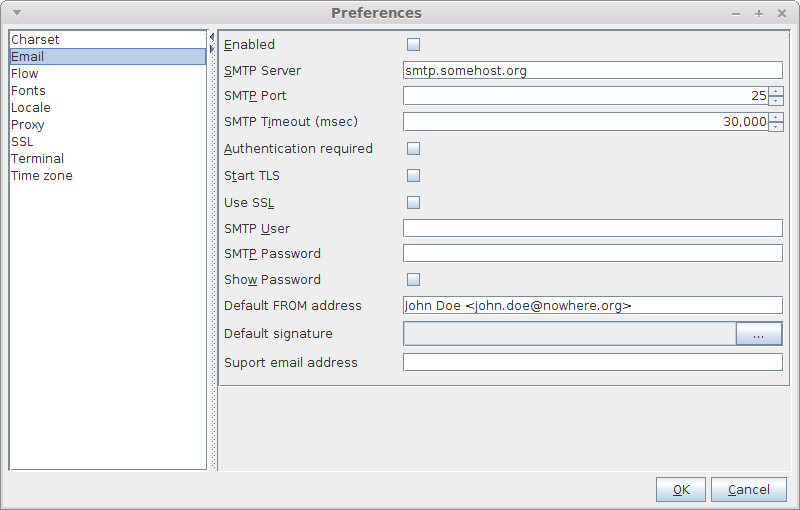
\includegraphics[width=10.0cm]{images/email_setup.png}
  \caption{Email preferences}
  \label{email_setup}
\end{figure}

\section{Actors}
The following standalone actors are available:
\begin{tight_itemize}
	\item \textit{SMTPConnection} -- for configuring a SMTP server connection.
\end{tight_itemize}
The following transformers are available:
\begin{tight_itemize}
	\item \textit{CreateEmail} -- creates an Email object. Interprets incoming files
	as attachments.
	\item \textit{EmailFileReader} -- reads email files with the specified email reader.
\end{tight_itemize}
The following sinks are available:
\begin{tight_itemize}
	\item \textit{EmailFileWriter} -- writes Email objects to files using the specified
	email writer.
	\item \textit{EmailViewer} -- displays an Email object; can be used in conjunction 
	with the \textit{DisplayPanelManager} as well.
	\item \textit{SendEmail} -- sends Email objects to a SMTP server.
\end{tight_itemize}

\heading{SMTPConnection}
If you do not want to store the password with the flow - after all, the password
is only obscured with base64 encoding - you can enable the 
\textit{promptForPassword} option. This will prompt the user with a dialog 
for entering a password to be used for the connection.

\section{Addressbook}
ADAMS also offers a very simple addressbook for emails. Figure \ref{email_address_book}
shows a screenshot of it.
\begin{figure}[htb]
  \centering
  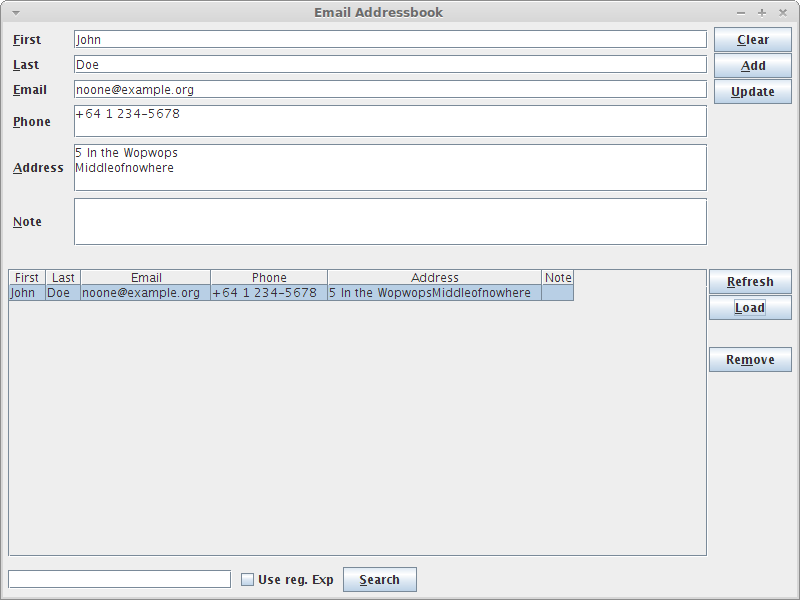
\includegraphics[width=10.0cm]{images/email_addressbook.png}
  \caption{Email address book}
  \label{email_address_book}
\end{figure}

\section{Command-line}
Using the \textit{adams.core.net.SimpleMailer} command-line tool, you can read
and send previously saved emails. The following command-line loads/sends all 
files in the directory \textit{/some/where} that end with \textit{.props} using the
\textit{PropertiesEmailFileReader} reader:
\begin{verbatim}
java -cp lib/* adams.core.net.SimpleMailer
  -env adams.env.Environment
  -reader adams.data.io.input.PropertiesEmailFileReader
  -watch-dir /some/where
  -regexp ".*.props"
  -D 1
\end{verbatim}
After a file got sucessfully loaded and sent, it gets (by default) the 
\textit{.sent} extension appended. If the process failed, the \textit{.failed}
extension is used (by default).
Use the \textit{-h} or \textit{-help} option on the command-line to list all 
the available options.

\section{Support email}
In order to make it easier for users or clients, you can set up a
\textit{support email}, which makes it easy to send through error reports.
These error reports get the \textit{system info} and current content
of the \textit{console window} automatically attached.

To enable this feature, configure the email setup through the preferences
and fill in a \textit{Support email address}. After the application has
been restarted, you get a \textit{Send error report} menu item in the
\textit{Program} menu and the \textit{Send error report} action in the flow's
notification area is enabled as well (this one also attaches the flow that
generated the error for further analysis).


%%%%%%%
% FTP %
%%%%%%%

\chapter{FTP}
In addition to Email, ADAMS also supports FTP (file transfer protocol). Since
FTP does not encrypt the commands or transferred data, it is recommended to not
use it outside a company's network or for non-anonymous access (e.g., download
from a public FTP server).

The following actors are available:
\begin{tight_itemize}
	\item \textit{FTPConnection} -- standalone actor that defines the server
	connection.
	\item \textit{FTPDisconnect} -- transformer that closes an existing 
	connection, to avoid too many open connections (simply passes through any 
	token it receives).
	\item \textit{FTPGet} -- for obtaining a remote file via FTP.
	\item \textit{FTPNoOp} -- sends a NOOP command to the server; useful when
	trying to keep the connection alive.
	\item \textit{FTPSend} -- for sending a file via FTP to a remote host.
\end{tight_itemize}
The \textit{FTPConnection} standalone allows you to enter the password at 
runtime, if you do not want to store the password with the
flow setup. At execution time, the user gets prompted with a dialog to enter
a password to be used for the connection.

There are also several \textit{searchlets} available for the
\textit{FileSystemSearch} source actor that allow the listing of remote
files.

%%%%%%%
% SSH %
%%%%%%%

\chapter{SSH}
ADAMS also comes with SSH support, thanks to the JSch library
\footnote{\url{http://www.jcraft.com/jsch/}{}}. This allows for secure remote
access. At the time of writing, RSA
\footnote{\url{http://en.wikipedia.org/wiki/RSA_\%28algorithm\%29}{}} and DSA
\footnote{\url{http://en.wikipedia.org/wiki/Digital_Signature_Algorithm}{}} are
supported for public key encryption schemes.

The following actors are available:
\begin{tight_itemize}
	\item \textit{SSHConnection} -- standalone actor that defines the server
	connection (user/password or public key authentication).
	\item \textit{SSHExec} -- for executing remote commands.
	\item \textit{ScpFrom} -- for copying a file \textit{from} a remote host using
	secure copy.
	\item \textit{ScpTo} -- for copying a file \textit{to} a remote host using
	secure copy.
	\item \textit{SFTPGet} -- for obtaining a remote file via secure FTP.
	\item \textit{SFTPSend} -- for sending a file via secure FTP to a remote host.
\end{tight_itemize}
The \textit{SSHConnection} standalone allows you to prompt the user as runtime
to enter a password, in case you do not want to store the connection's password
with the flow setup. The user has to enter the password through a dialog that
pops up when the flow gets executed.

There are also several \textit{searchlets} available for the
\textit{FileSystemSearch} source actor that allow the listing of remote
files.

%%%%%%%
% SSL %
%%%%%%%

\chapter{SSL}
How ADAMS handles SSL, e.g., for HTTPS connections, can be configured in the
\textit{SSL} preferences. Figure \ref{ssl_setup} shows a screenshot of the
default settings.

\begin{figure}[htb]
  \centering
  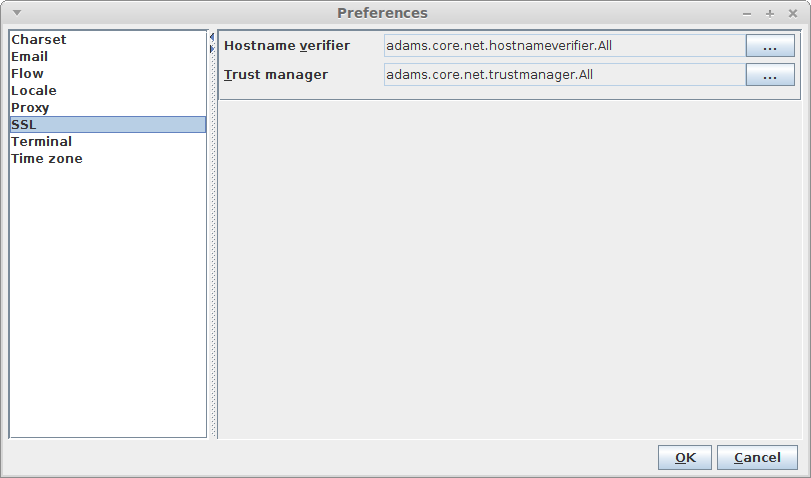
\includegraphics[width=10.0cm]{images/ssl_setup.png}
  \caption{SSL preferences}
  \label{ssl_setup}
\end{figure}

%%%%%%%
% SMB %
%%%%%%%

\chapter{SMB}
What WINS server ADAMS uses for SMB (i.e., Windows shares), can be configured in the
\textit{SMB} preferences. Figure \ref{smb_setup} shows a screenshot of the
default settings.

\begin{figure}[htb]
  \centering
  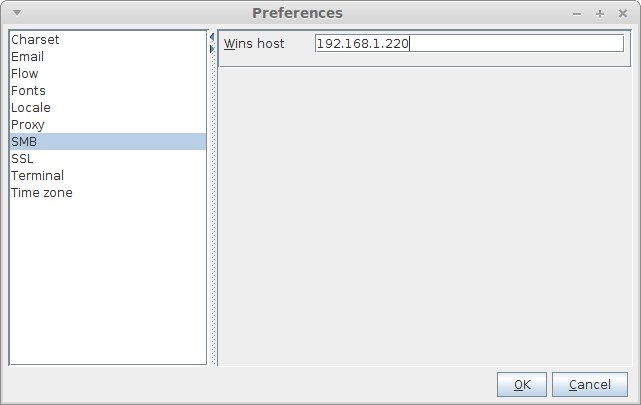
\includegraphics[width=10.0cm]{images/smb_setup.png}
  \caption{SMB preferences}
  \label{smb_setup}
\end{figure}

The following actors are available:
\begin{tight_itemize}
	\item \textit{SMBConnection} -- standalone actor that defines the server
	connection (domain/user/password).
	\item \textit{SMBGet} -- for obtaining a remote file from a Windows host.
	\item \textit{SMBSend} -- for sending a file to a remote Windows host.
\end{tight_itemize}

There are also several \textit{searchlets} available for the
\textit{FileSystemSearch} source actor that allow the listing of remote
files.

%%%%%%%%%%%%%%%%%%%
% Remote commands %
%%%%%%%%%%%%%%%%%%%

\chapter{Remote commands}

The \textit{adams-net} module adds several connection schemes for the
remote command framework:

\begin{tight_itemize}
	\item \textit{FTPConnection} -- sends commands as files via FTP.
	\item \textit{ScpConnection} -- sends commands as files using secure
	copy (\textit{scp}).
	\item \textit{SSHConnection} -- offers SSH tunnelling, useful when
	remote servers are locked down.
\end{tight_itemize}


%%%%%%%%
% Misc %
%%%%%%%%

\chapter{Miscellaneous}
Some other basic, but useful actors are the following:
\begin{tight_itemize}
	\item \textit{Browser} -- opens the system's default browser with the specified
	URL.
	\item \textit{DownloadFile} -- downloads a file via HTTP and saves it to disk.
	\item \textit{DownloadContent} -- downloads (textual) content via HTTP and 
	forwards it.\footnote{adams-net-download\_content.flow}
	\item \textit{HTMLFileReader} -- reads an HTML file, generating a DOM object.
	\item \textit{HttpRequest} -- the source allows accessing URLs (POST/GET, sending data,
	cookies), returns the HTML from the reponse as text; the transformer allows
	sending the incoming text via HTTP request (and optional headers).
	\item \textit{MimeType} -- determines the mime-type of
	files.\footnote{adams-net-mimetype.flow}
	\item \textit{Socket} -- source and sink allow you to receive and send
	strings and byte arrays via sockets.
	\item \textit{URLSupplier} -- outputs one or more URLs.
	\item \textit{WebServer} -- simple web server for serving static files.
	\item \textit{WebSocketClient} -- allows executing of clients that implement
	the websocket protocol\footnote{\url{https://en.wikipedia.org/wiki/WebSocket}{}}.
	\item \textit{WebSocketServer} -- allows running of websocket servers.
\end{tight_itemize}
The following conversions are available:
\begin{tight_itemize}
    \item \textit{HTMLToDOM} -- generates a DOM document from an HTML string.
    \item \textit{HTMLToText} -- extracts the text from an HTML string.
    \item \textit{RenderHTMLAsText} -- renders an HTML string as text.
	\item \textit{SpreadSheetToHTML} -- converts a spreadsheet into an HTML 
	page (or just a table fragment).
	\item \textit{StringToURL} -- converts a string into a URL object.
	\item \textit{URLToString} -- converts a URL object into a string.
\end{tight_itemize}
In case you need to debug a connection, \texttt{telnet} is always a useful tool.
ADAMS comes with a very simple graphical version, depicted in Figure \ref{telnet}.
\begin{figure}[htb]
  \centering
  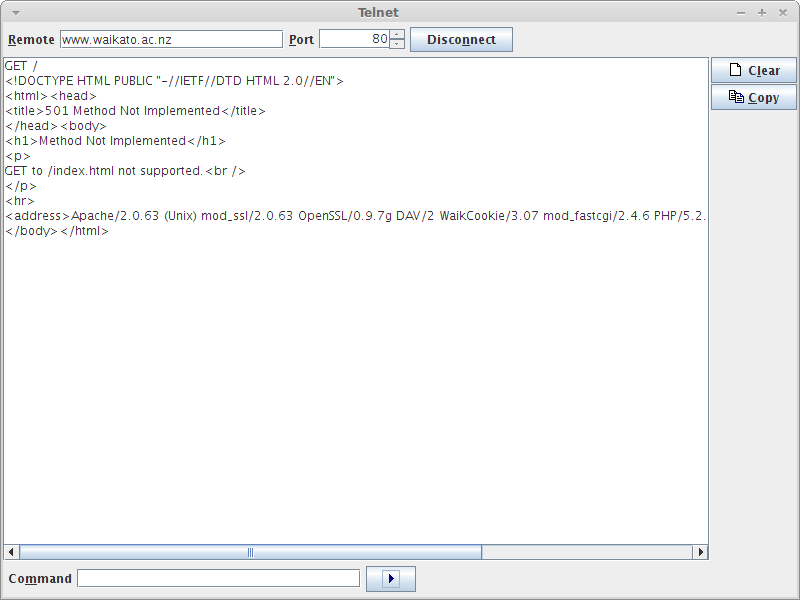
\includegraphics[width=8.0cm]{images/telnet.png}
  \caption{Telnet dialog}
  \label{telnet}
\end{figure}


%%%%%%%%%%%%%%%%%%%%%%%%%%%%%%%%%%%
% Copyright (c) 2009-2012 by the University of Waikato, Hamilton, NZ. 
% This work is made available under the terms of the 
% Creative Commons Attribution-ShareAlike 4.0 license,
% http://creativecommons.org/licenses/by-sa/4.0/.
%
% Version: $Revision$

\begin{thebibliography}{999}
	% to make the bibliography appear in the TOC
	\addcontentsline{toc}{chapter}{Bibliography}

    % references
	\bibitem{adams}
		\textit{ADAMS} -- Advanced Data mining and Machine learning System \\
		\url{https://adams.cms.waikato.ac.nz/}{}

	\bibitem{esrigrid}
	 	\textit{Esri Grid} -- a raster GIS file format deveoped by Esri. \\
		\url{https://en.wikipedia.org/wiki/Esri\_grid}{}

	\bibitem{kml}
	 	\textit{Keyhole Markup Language} -- an XML notation for expressing
	 	geographic annotation and visualization within Internet-based,
	 	two-dimensional maps and three-dimensional Earth browsers. \\
		\url{http://en.wikipedia.org/wiki/Keyhole\_Markup\_Language}{}

	\bibitem{postgresql}
	 	\textit{PostgreSQL} -- a powerful, open source object-relational
	 	database system. \\
		\url{http://www.postgresql.org/}{}

	\bibitem{postgis}
		\textit{PostGIS} -- a spatial database extender for PostgreSQL
		object-relational database. It adds support for geographic
		objects allowing location queries to be run in SQL.  \\
		\url{http://postgis.net/}{}

	\bibitem{srid4269}
	 	\textit{SRID 4269} -- or NAD 83 (North American Datum). \\
		\url{http://spatialreference.org/ref/epsg/4269/}{}

	\bibitem{mysql}
		\textit{MySQL} -- an open-source relational database management
		system (RDBMS) \\
		\url{http://www.mysql.com/}{}

\end{thebibliography}


\end{document}
